\documentclass[journal]{IEEEtran}

\usepackage{cite}
\usepackage{amsmath,amssymb}
\usepackage{graphicx}
\usepackage{booktabs}
\usepackage{multirow}
\usepackage{url}
\usepackage[hidelinks]{hyperref}
\usepackage{array}
\usepackage{tikz}
\usetikzlibrary{arrows.meta,positioning,fit,backgrounds,calc}
\definecolor{gb}{HTML}{4A5A6E}   % dull dark grey blue, the colour of all diagrams and graphs

\graphicspath{{figures/}}

\begin{document}

\title{Forecast-Driven Model Predictive Control with Reinforcement Learning for Low-Carbon Community Battery Scheduling}

\author{Elena~Margaret~Ellis, Anora~V and Cherish~Vasant}

\markboth{}{}

\maketitle

\begin{abstract}
\boldmath
Home batteries can cut electricity bills and emissions by shifting consumption in time, but a controller in a real
building never knows the future demand, solar generation or carbon intensity. We propose an \emph{RL-tuned model
predictive controller} for the batteries of a whole district. Gradient-boosted forecasters predict the load and solar
output of every building, and a linear program uses these forecasts to plan all batteries over the next 30 hours. A
reinforcement learning (RL) agent, trained with Truncated Quantile Critics (TQC), sets three weights of this program
every hour. Its reward adds up to the official performance indicators. Because the agent sees only district-level
features, one policy trained on five buildings controls districts of any size. We evaluate the controller on the
CityLearn Challenge 2022 benchmark with the official formulas, on all 17 buildings and with three seeds. It lowers the
electricity cost by 34.3\% and the emissions by 22.2\% in the training district. Its Phase~III public score is
$0.774 \pm 0.003$ and its private score $0.844 \pm 0.004$, which places it 8th among the 42 public entries (winner
0.728). Its carbon score of 0.764 is the lowest of all 42 entries. Our ablations show that the optimiser, the forecasts
and the RL tuning all contribute.
\end{abstract}

\begin{IEEEkeywords}
Battery energy storage, demand response, deep reinforcement learning, model predictive control, truncated quantile
critics, load forecasting, reward design, CityLearn, carbon-aware control, grid-interactive buildings.
\end{IEEEkeywords}

\section{Introduction}
\IEEEPARstart{B}{uildings} use a large share of all electricity, and rooftop photovoltaic (PV) panels and home
batteries now turn many of them into flexible grid resources. A battery that charges when power is cheap or clean, and
discharges when it is costly or carbon-intensive, lowers both the owner's bill and the emissions caused by the home. A
fleet of such batteries can also smooth the load that the local grid has to supply
\cite{vazquez2019review,wang2020rlbuildings}. This is not easy. Demand, solar output and carbon intensity all
change by the hour, and a charge decision made now affects what the battery can do many hours later.

Two families of controllers are common. Rule-based controllers are simple, but they cannot adapt to the weather, the
tariff or the state of the grid. Model predictive control (MPC) plans ahead with forecasts, yet it is only as good as
those forecasts and as the fixed weights that trade cost against emissions and grid impact. Model-free deep
reinforcement learning (RL) \cite{sutton2018rl} learns a policy from interaction alone
\cite{yu2021review,nagy2023tenquestions}. An RL agent on its own, however, must discover the daily patterns of price and
demand, and the long-term effect of each charge decision, from a single scalar reward. The CityLearn environment
\cite{vazquez2019citylearn,nweye2024citylearn} and the NeurIPS 2022 CityLearn Challenge \cite{citylearn2022challenge}
turned this problem into a shared benchmark, whose score combines the electricity cost, the carbon emissions and two
grid key performance indicators (KPIs).

In this paper we combine the two ideas. Gradient-boosted models forecast the load and PV of each home, and a linear
program turns these forecasts into a battery schedule that respects the battery limits. An RL agent then adjusts the trade-offs
of the program every hour, so that it can correct for what fixed weights and imperfect forecasts miss. We call the
result an \emph{RL-tuned MPC} (Fig.~\ref{fig:arch}).

Our first contribution is this controller, in which a TQC agent sets three weights of a receding-horizon linear program
every hour. Since its inputs are district-level, one policy runs on districts of any size. Our second contribution is a
\emph{score-aligned counterfactual reward}, whose terms add up to the official KPIs, use the no-battery run as their
scale and measure the gain over idle batteries. Third, we evaluate the controller in full. We score all 17 challenge
homes with the official formulas over three seeds and compare them with all 42 public leaderboard entries and with the
private medians. We also ablate each component and show which forecast errors limit the score.

The rest of the paper is organised as follows. Section~\ref{sec:related} reviews the literature, and
Section~\ref{sec:problem} states the problem. In Section~\ref{sec:method} we describe the controller, and in
Section~\ref{sec:setup} the experiments. Section~\ref{sec:results} reports the results, Section~\ref{sec:discussion}
discusses them and Section~\ref{sec:conclusion} concludes.

\section{Literature Review}\label{sec:related}

\subsection{Reinforcement Learning for Building Energy}
V\'azquez-Canteli and Nagy \cite{vazquez2019review} reviewed RL for demand response and found that most studies used
simple function approximators, single homes and custom simulators, so their results were hard to compare. Wang and
Hong \cite{wang2020rlbuildings} and Yu \emph{et al.} \cite{yu2021review} surveyed deep RL for building control and named
sample efficiency, safety, reward design and transfer across homes as the main open problems. Nagy \emph{et al.}
\cite{nagy2023tenquestions} raised ten questions on RL for building energy, among them the need for shared benchmarks
and KPIs. Dulac-Arnold \emph{et al.} \cite{dulacarnold2021challenges} listed the challenges of real-world RL, and three of
them, namely multi-objective rewards, partial observability and limited data, are central to battery control. We
address all three.

\subsection{CityLearn and Grid-Interactive Communities}
CityLearn \cite{vazquez2019citylearn} is an OpenAI Gym environment for demand response in districts of homes with
storage and PV. Its second version \cite{nweye2024citylearn} adds electric vehicles, occupant comfort, resilience and
carbon-aware control. MARLISA \cite{vazquez2020marlisa} coordinated several agents through sequential action selection
to shape the district load, while Nweye \emph{et al.} \cite{nweye2022realworld} studied the real-world challenges
of multi-agent RL in such communities. The NeurIPS 2022 CityLearn Challenge \cite{citylearn2022challenge} scored
controllers on cost, carbon and grid KPIs, each divided by its value with no batteries. We use its data, its KPIs and
its leaderboards as our references.

\subsection{Forecasting, Optimisation and the Challenge Winners}
MPC solves an optimisation problem over a moving horizon of forecasts and applies only the first decision
\cite{rawlings2017mpc}. The organisers' overview \cite{nweye2023challenge} shows that all top entries of the 2022
challenge combined forecasting with optimisation or learning. The winner, Together, forecast load and PV with
gradient-boosted trees and linear models and then mixed a rolling-horizon stochastic optimiser with multi-agent PPO
\cite{yu2022mappo}. The runner-up used dynamic programming in the first phase and, later, forecasts with a small policy
network trained by CMA-ES \cite{hansen2016cma}. CUFE, in third place, solved a 24-hour linear program per building with
linear forecasts, while DivMARL averaged a shared SAC policy with a rule driven by XGBoost forecasts. Like the winner,
we forecast with gradient-boosted trees, here LightGBM \cite{ke2017lightgbm} with settings chosen by Optuna
\cite{akiba2019optuna}.

\subsection{Deep RL for Continuous Control}
The MPC weights are continuous, so actor-critic methods fit the task. DDPG \cite{lillicrap2016ddpg} and TD3
\cite{fujimoto2018td3} learn deterministic policies with off-policy critics, and TD3 adds clipped double Q-learning to
limit over-estimation. Soft Actor-Critic (SAC) \cite{haarnoja2018sac} maximises the reward plus the policy entropy and
tunes its temperature automatically. PPO \cite{schulman2017ppo} is a common on-policy alternative. We use TQC
\cite{kuznetsov2020tqc}, which extends SAC with a mixture of distributional critics and drops their largest quantiles
to reduce over-estimation. All agents come from the Stable-Baselines3 library \cite{raffin2021sb3}.

\subsection{Reward Design}
Battery control has several objectives \cite{roijers2013survey}, such as cost, emissions, ramping and peaks, which often
conflict with each other, so a single reward needs weights and scales for all of them. If the scales are poor, one objective dominates the others. Ng
\emph{et al.} \cite{ng1999shaping} showed which changes to a reward leave the optimal policy unchanged. Our counterfactual
baseline relies on this result. For storage arbitrage, Cao \emph{et al.} \cite{cao2020arbitrage} showed that a
degradation model in the reward changes the learned strategy. This motivates the small battery-wear term in our reward.

\subsection{Evaluation of RL Results}
Henderson \emph{et al.} \cite{henderson2018matters} and Agarwal \emph{et al.} \cite{agarwal2021precipice} showed that
deep RL results vary strongly with the random seed. A single run can therefore mislead. We report the proposed
controller as the mean and standard deviation of three seeds, and we evaluate each seed without exploration over a full
year.

\section{Problem Formulation}\label{sec:problem}

\subsection{Environment}
We use CityLearn 2.1.2 with the data of the 2022 challenge, which contains 17 homes in three districts: five public
training buildings (1--5), five validation buildings (6--10) and seven test buildings (11--17). Each home has a load it
cannot shift, rooftop PV and one battery of 6.4\,kWh and 5\,kW. The simulation runs hourly for one year, or 8{,}759
control steps, and every hour our controller sets the charge or discharge rate of each battery as a fraction of its
capacity. The decision acts over the following hour. Power is billed with a time-of-use tariff. The carbon
intensity of the grid changes over the day.

\subsection{Information Available to the Controller}
At each hour the controller sees the month, the day type and the hour. It also sees the outdoor temperature, the
humidity and the diffuse and direct solar irradiance, each with the environment's 6, 12 and 24-hour forecasts, and the
current carbon intensity. For each home it sees the load, the PV output, the battery state of charge (SoC) and the net
consumption. Finally, it sees the current price with its 6, 12 and 24-hour values from the tariff. We use only these
signals, together with their past values.

\subsection{Key Performance Indicators}
Let $E_t$ be the district's net consumption at hour $t$ (positive for imports), $\pi_t$ the price and $I_t$ the carbon
intensity. We mark the same quantity in the run without batteries with a superscript ``nb''. The official KPIs are
\begin{align}
  C &= \frac{\sum_t \max(0, E_t \pi_t)}{\sum_t \max(0, E_t^{\mathrm{nb}} \pi_t)}, \qquad
  G = \frac{\sum_t \max(0, E_t I_t)}{\sum_t \max(0, E_t^{\mathrm{nb}} I_t)}, \\
  R &= \frac{\sum_t |E_t - E_{t-1}|}{\sum_t |E_t^{\mathrm{nb}} - E_{t-1}^{\mathrm{nb}}|}, \qquad
  D = \tfrac{1}{2}\bigl(R + (1-L)\bigr),
\end{align}
where $C$ is the cost, $G$ the carbon emissions, $R$ the ramping and $1-L$ the mean monthly value of $1 - \bar E / \max E$
relative to no battery. The grid KPI $D$ averages the last two. Exports earn nothing. Since the clipping applies to
the district total, one home's export can offset another's import within the same hour. All KPIs are ratios to the no-battery run.
Values below one are gains.

The score of a district $d$ is $S_d=(C+G+D)/3$. The first phase of the challenge ranked entries by $(C+G)/2$ on the
training buildings, which we call the Phase~I score. The final phase ranked them by a \emph{public} score
$0.4\,S_\mathrm{train} + 0.6\,S_\mathrm{val}$, and it chose the winners by a \emph{private} score
$0.2\,S_\mathrm{train} + 0.3\,S_\mathrm{val} + 0.5\,S_\mathrm{test}$ \cite{nweye2023challenge}. We report all three
scores, with the public one as our main measure.

\section{Proposed Methodology}\label{sec:method}

\begin{figure*}[!t]
\centering
\resizebox{\textwidth}{!}{%
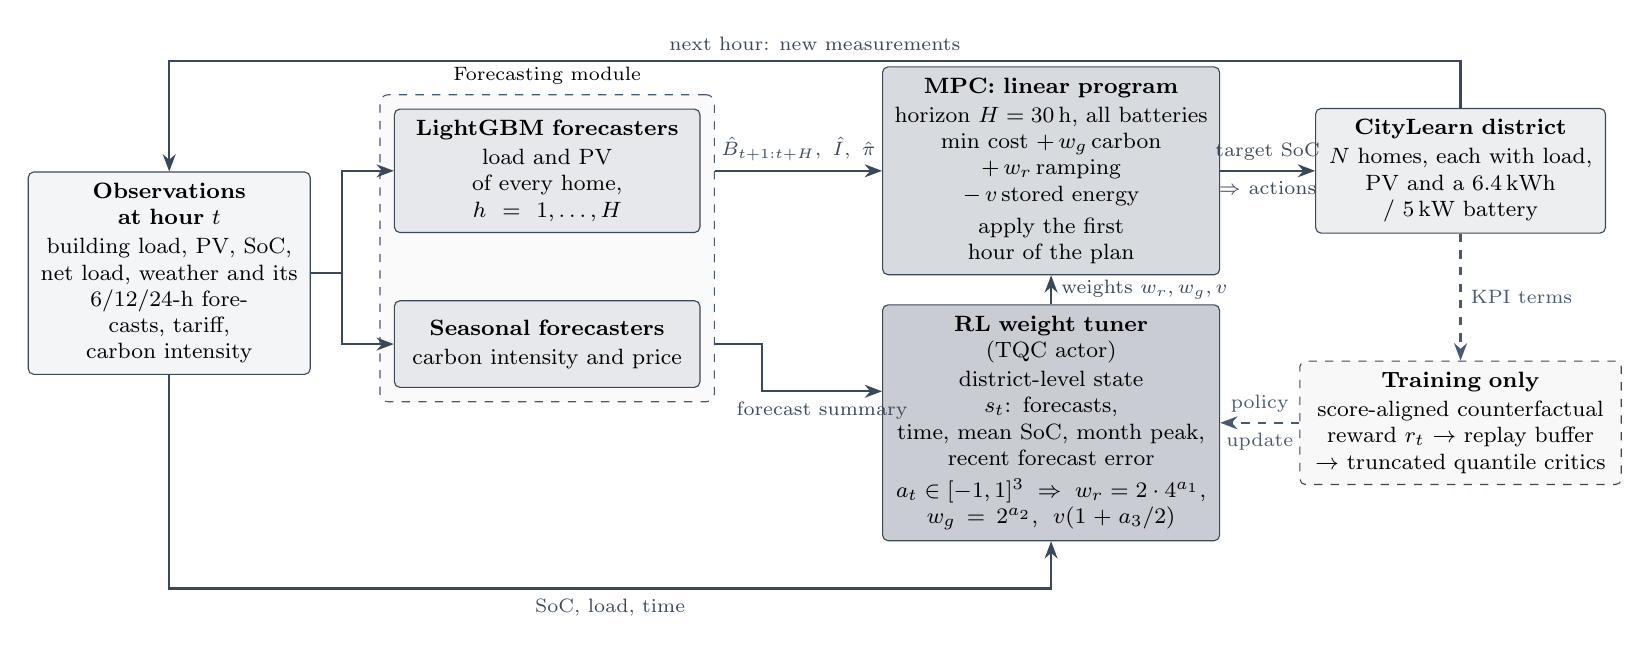
\begin{tikzpicture}[
  font=\footnotesize, >={Stealth[length=2.2mm]},
  box/.style={draw=gb!80!black, rounded corners=2pt, align=center, inner sep=4pt, minimum height=11mm, fill=white},
  obs/.style={box, fill=gb!6, text width=33mm},
  fc/.style={box, fill=gb!14, text width=36mm},
  rl/.style={box, fill=gb!30, text width=40mm},
  opt/.style={box, fill=gb!22, text width=40mm},
  env/.style={box, fill=gb!10, text width=34mm},
  train/.style={box, dashed, fill=gb!4, text width=38mm},
  lab/.style={font=\scriptsize, align=center},
  flow/.style={->, thick, gb!80!black},
  tflow/.style={->, thick, dashed, gb}]

\node[obs] (obs) at (0,0) {\textbf{Observations at hour $t$}\\[1pt] building load, PV, SoC,\\ net load, weather and its\\
  6/12/24-h forecasts, tariff,\\ carbon intensity};
\node[fc] (lgb) at (4.8,1.3) {\textbf{LightGBM forecasters}\\[1pt] load and PV of every home,\\
  $h = 1,\dots,H$};
\node[fc] (seas) at (4.8,-0.9) {\textbf{Seasonal forecasters}\\[1pt] carbon intensity and price};
\begin{scope}[on background layer]
\node[draw=gb, dashed, rounded corners=3pt, fill=gb!3, inner sep=5pt, fit=(lgb)(seas),
      label={[lab]above:Forecasting module}] (fcm) {};
\end{scope}
\node[opt] (mpc) at (11.2,1.3) {\textbf{MPC: linear program}\\[1pt]
  horizon $H = 30$\,h, all batteries\\ min cost $+\,w_g$\,carbon $+\,w_r$\,ramping\\ $-\,v$\,stored energy\\[2pt]
  apply the first hour of the plan};
\node[rl] (actor) at (11.2,-1.9) {\textbf{RL weight tuner} (TQC actor)\\[1pt]
  district-level state $s_t$: forecasts,\\ time, mean SoC, month peak,\\ recent forecast error\\[2pt]
  $a_t \in [-1,1]^3 \;\Rightarrow\; w_r = 2\cdot 4^{a_1},$\\ $w_g = 2^{a_2},\; v(1 + a_3/2)$};
\node[env] (envn) at (16.4,1.3) {\textbf{CityLearn district}\\[1pt] $N$ homes, each with load,\\ PV and a
  6.4\,kWh / 5\,kW battery};
\node[train] (critic) at (16.4,-1.9) {\textbf{Training only}\\[1pt] score-aligned counterfactual\\ reward $r_t$
  $\rightarrow$ replay buffer\\ $\rightarrow$ truncated quantile critics};

% data flow
\draw[flow] (obs.east) -- ++(4mm,0) |- (lgb.west);
\draw[flow] (obs.east) -- ++(4mm,0) |- (seas.west);
\draw[flow] (lgb.east -| fcm.east) -- node[lab, above]{$\hat B_{t+1:t+H},\ \hat I,\ \hat\pi$} (lgb.east -| mpc.west);
\draw[flow] (seas.east -| fcm.east) -- ++(6mm,0) |- node[lab, pos=0.75, below]{forecast summary} ([yshift=4mm]actor.west);
\draw[flow] (actor.north) -- node[lab, right]{weights $w_r, w_g, v$} (mpc.south);
\draw[flow] (mpc.east) -- node[lab, above]{target SoC}node[lab, below]{$\Rightarrow$ actions} (envn.west);
\draw[flow] (envn.north) -- ++(0,6mm) -| node[lab, pos=0.25, above]{next hour: new measurements} (obs.north);
\draw[flow] (obs.south) |- node[lab, pos=0.75, below]{SoC, load, time} ([yshift=-6mm]actor.south) -- (actor.south);
% training flow
\draw[tflow] (envn.south) -- node[lab, right]{KPI terms} (critic.north);
\draw[tflow] (critic.west) -- node[lab, above]{policy}node[lab, below]{update} (actor.east);
\end{tikzpicture}}
\caption{Architecture of the proposed RL-tuned MPC. Every hour, the forecasters predict the next $H$ hours. The
RL agent maps a district-level state to three weights of a linear program, and the first hour of the program's plan is
applied to the batteries. Dashed parts are used only during training.}
\label{fig:arch}
\end{figure*}

The controller in Fig.~\ref{fig:arch} repeats the same cycle every hour. It first forecasts the next $H = 30$ hours,
after which the RL agent sets three weights from a small district-level state. A linear program, which we call the
solver, uses these weights to plan all batteries over the horizon. Only the first hour of the plan is applied. The
cycle then starts again an hour later, and we describe its three parts below.

\subsection{Forecasting Module}\label{sec:fc}
Each hour we forecast every home's load and PV output, the carbon intensity and the price for the next $H$ hours. One
LightGBM model \cite{ke2017lightgbm} per quantity covers all horizons and homes. Its inputs are recent and lagged
values, the mean of the same hour over the past seven days, the calendar, the current weather and the environment's
weather forecast for the target hour. We divide each value input by the home's mean absolute value over the past week,
so that a model trained on some homes also applies to others. The model for a district is trained on the homes of the
other two districts, and Optuna \cite{akiba2019optuna} chooses its settings by cross-validation between them.

Carbon intensity and price follow simple seasonal rules. For carbon, we average the same hour yesterday and over the
last week and add the current error, which decays as $0.8^h$ over the horizon. For price, we repeat the tariff of the
same hour one week earlier. Both rules are cheap to compute. The tariff, in fact, repeats exactly from week to week.

\subsection{Receding-Horizon Linear Program}\label{sec:mpc}
Our MPC receives the forecast net load of the district $\hat B_h$ (load minus PV), the prices $\hat\pi_h$ and the carbon
intensities $\hat I_h$. It then solves
\begin{equation}
\begin{split}
\min\; & \sum_{h=1}^{H} \Bigl(\tfrac{\hat\pi_h}{\bar c} + w_g \tfrac{\hat I_h}{\bar g}\Bigr) m_h
        + \tfrac{w_r}{2\bar r} \sum_{h=1}^{H} \rho_h - v\,\eta \sum_b s_{b,H} \\
\text{s.t. } & m_h \ge \hat B_h + \textstyle\sum_b (x^+_{b,h} - x^-_{b,h}),\; m_h \ge 0, \\
& \rho_h \ge |E_h - E_{h-1}|,\; E_h = \hat B_h + \textstyle\sum_b (x^+_{b,h} - x^-_{b,h}), \\
& s_{b,h} = s_{b,h-1} + \eta x^+_{b,h} - x^-_{b,h}/\eta,\; 0 \le s_{b,h} \le 6.4, \\
& 0 \le x^\pm_{b,h} \le \min(5,\ 21 - 3.125\, s_{b,h-1}),
\end{split}
\label{eq:lp}
\end{equation}
where $m_h$ is the district import, $\rho_h$ the ramp and $s_{b,h}$ the energy stored in battery $b$. The charge and
discharge powers are $x^\pm_{b,h}$, with an efficiency of $\eta=\sqrt{0.9}$ each way, and they are
limited to 5\,kW. With the last constraint we model
CityLearn's power taper above 80\% charge. The running no-battery means $\bar c$, $\bar g$ and $\bar r$ put cost, carbon
and ramping on the scale of the KPIs. The weight $v$ is the median unit cost over the horizon and gives a value to
the energy left at its end. Exports earn nothing, so only imports are priced.

We apply only the first hour of the plan, by moving each battery to its planned state of charge. One hour later the
problem is solved again with new forecasts (Fig.~\ref{fig:horizon}). With the HiGHS solver, each problem takes about
20\,ms. A full simulated year therefore needs less than four minutes of solver time.

\begin{figure}[!t]
\centering
\resizebox{\columnwidth}{!}{%
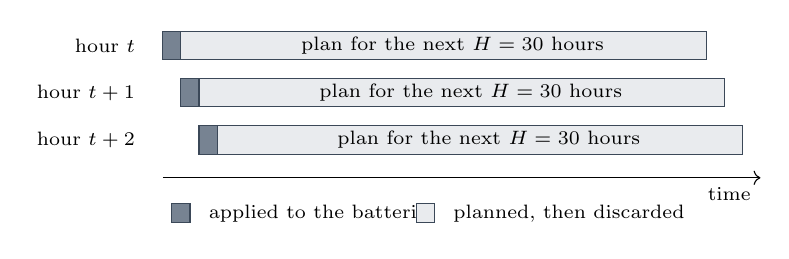
\begin{tikzpicture}[font=\scriptsize, x=2.3mm, y=6mm]
\foreach \r/\s/\lab in {0/0/hour $t$, 1/1/hour $t+1$, 2/2/hour $t+2$} {
  \node[anchor=east] at (-1,-\r) {\lab};
  \draw[draw=gb!80!black, fill=gb!12] (\s,-\r-0.3) rectangle (\s+30,-\r+0.3);
  \draw[draw=gb!80!black, fill=gb!75] (\s,-\r-0.3) rectangle (\s+1,-\r+0.3);
  \node at (\s+16,-\r) {plan for the next $H = 30$ hours};
}
\draw[->] (0,-2.8) -- (33,-2.8) node[below left] {time};
\draw[draw=gb!80!black, fill=gb!75] (0.5,-3.75) rectangle (1.5,-3.35); \node[anchor=west] at (2,-3.55) {applied to the batteries};
\draw[draw=gb!80!black, fill=gb!12] (14,-3.75) rectangle (15,-3.35); \node[anchor=west] at (15.5,-3.55) {planned, then discarded};
\end{tikzpicture}}
\caption{Receding horizon. Every hour the linear program plans 30 hours ahead with fresh forecasts and weights, and
only the first hour is carried out.}
\label{fig:horizon}
\end{figure}

\subsection{RL Weight Tuner}\label{sec:tuner}
Fixed weights in (\ref{eq:lp}) cannot adapt to the season, the forecast quality or the battery state, so we let an RL
agent output three numbers $a_t \in [-1,1]^3$ every hour. They set the ramp weight $w_r = 2\cdot 4^{a_1}$, the
carbon weight $w_g = 2^{a_2}$ and the end-of-horizon value $v(1 + a_3/2)$. Each weight is centred on a good fixed
setting. An action of zero is thus already sound. The agent's state holds the forecasts of net load,
carbon intensity and price over the horizon, the time of day and season, the mean state of charge, the current load
and month peak, and the latest forecast error. None of these depends on the number of homes. A policy trained on five
homes can therefore control the seven test homes as well.

The agent learns from a \emph{score-aligned counterfactual reward}, built so that its terms add up exactly to the
numerators of the official KPIs, on their scale. At hour $t$ we use the district's clipped cost and emissions and its ramp,
\begin{equation}
\begin{gathered}
  \hat c_t = \frac{\max(0, E_t\pi_t)}{\bar c^{\,\mathrm{nb}}}, \qquad
  \hat g_t = \frac{\max(0, E_t I_t)}{\bar g^{\,\mathrm{nb}}}, \\
  \hat r_t = \frac{|E_t - E_{t-1}|}{\bar r^{\,\mathrm{nb}}},
\end{gathered}
\end{equation}
where a bar marks the mean of the term per step in the no-battery run. Then $\sum_t \hat c_t = T\cdot C$, so the return
over a year is a linear function of the KPIs. The peak term $\hat p_t$ is the rise of the running daily
maximum of $E_t$. The first hour of each day counts its full load, so the terms of a day add up to that day's peak. The
wear term is $\hat b_t = \sum_i |\mathrm{SoC}_{i,t}-\mathrm{SoC}_{i,t-1}|$. The reward is
\begin{equation}
  \begin{split}
  r_t = &-\bigl(\hat c_t + w_g\hat g_t + w_r\hat r_t + w_p\hat p_t + w_b\hat b_t\bigr) \\
        &+ \bigl(\hat c^{\,\mathrm{nb}}_t + w_g\hat g^{\,\mathrm{nb}}_t + w_r\hat r^{\,\mathrm{nb}}_t + w_p\hat p^{\,\mathrm{nb}}_t\bigr).
  \end{split}
  \label{eq:reward}
\end{equation}
The second bracket holds the same terms for the case in which the batteries stayed idle in that hour. Since it depends
only on outside data, and not on the actions or the battery state, it leaves the optimal policy unchanged
\cite{ng1999shaping}. It does, however, remove most of the variation caused by demand. The agent is thus rewarded for
the \emph{improvement} it causes, and a reward of zero means ``as good as no battery''. A real system can compute this
baseline online from the measured net load and the battery's own power.

We choose the weights to follow the score $S=(C+G+(R+1-L)/2)/3$. Cost has weight 1, ramping and peak have $w_r = w_p = 0.5$, and wear
has $w_b=0.1$. The peak term stands in for the load factor at each step, while the carbon weight of $w_g = 2$ puts extra weight on
emissions.

We train the agent with TQC \cite{kuznetsov2020tqc}, which has an actor and two distributional critics with 25
quantiles each. When the target is formed, the two largest quantiles of each critic are dropped. This limits the
over-estimation that a noisy, long-horizon reward invites. We train on the training district only. At
evaluation, the actor acts deterministically.

\section{Experimental Setup}\label{sec:setup}
We train the tuner for 100{,}000 environment steps, about 11.4 simulated years, on the five training buildings, with a
learning rate of $3\cdot10^{-4}$, a replay buffer of 200{,}000 transitions and a batch size of 256. We use
$\tau=0.005$, $\gamma=0.99$, one gradient step per environment step, 1{,}000 warm-up steps and automatic entropy tuning.
The actor and each critic have two hidden layers of 64 units, and we run three seeds (42, 100 and 2026) and report
the mean and standard deviation.

For evaluation, the trained policy runs on each district for the full year without retraining. We compute the KPIs
against the no-battery run on the same homes and, because CityLearn 2.1.2 contains all 17 homes, we can compute the
public and private scores ourselves with the official formulas. These are not the scores of the challenge's own evaluator.
As references we use no battery, where every KPI equals one, and the rule-based controller (RBC) supplied with
CityLearn.

To measure what each part contributes, we run ablations that change one part of the controller at a time and keep the
same protocol. We replace the RL tuner
with the best fixed weights we found (ramp weight 3, carbon weight 1, 24-hour horizon). We try horizons of 24 and
36 hours. We replace the tuned LightGBM settings with the defaults, and the LightGBM load and PV forecasts with seasonal
ones. We use SAC instead of TQC. Last, we remove the solver: a TQC agent with the same reward then sets the battery
rates directly, from the observations plus past-only history features, over 200{,}000 steps. Ablations with one seed use
seed 42.

\section{Results}\label{sec:results}

\subsection{Main Results}
We find that the controller improves every KPI in every district (Table~\ref{tab:main}, Fig.~\ref{fig:kpis}). On buildings 1--5
it lowers the cost by 34.3\% and the emissions by 22.2\% relative to no battery. It also smooths the district
load, with $R = 0.823$, $1-L = 0.977$ and $D = 0.900$. The RBC does worse than idle batteries on every KPI. It charges and discharges on a fixed schedule that ignores the
tariff, the carbon intensity and the PV.

We see the same gains in the validation district, where the cost falls by 34.5\% and the emissions by 24.5\%. The scores of the training and validation districts are almost equal, at $S = 0.778$ and
0.771, which shows that the controller is not fitted to the homes it was trained on. The seven test buildings differ
most from the training ones and gain less ($S = 0.914$), with the cost down by 19.9\% and the emissions by 4.1\%. All
three seeds agree closely. No score varies by more than 0.006.

\begin{table}[!t]
\centering
\caption{The proposed RL-tuned MPC in each district. Indicators relative to no battery (lower is better), mean of three
seeds, $\pm$ standard deviation for the scores. The policy is trained on the training buildings only.}
\label{tab:main}
\setlength{\tabcolsep}{3pt}
\resizebox{\columnwidth}{!}{%
\begin{tabular}{@{}llccccc@{}}
\toprule
District & Controller & $C$ & $G$ & $D$ & Phase I & $S$ \\
\midrule
\multirow{3}{*}{Train (1--5)} & No battery & 1.000 & 1.000 & 1.000 & 1.000 & 1.000 \\
                              & RBC        & 1.070 & 1.193 & 1.075 & 1.132 & 1.113 \\
                              & RL-tuned MPC & \textbf{0.657} & \textbf{0.778} & \textbf{0.900} &
                                \textbf{0.717}{\scriptsize$\pm$.002} & \textbf{0.778}{\scriptsize$\pm$.002} \\
\midrule
Validation (6--10) & RL-tuned MPC & 0.655 & 0.755 & 0.904 & 0.705 & 0.771{\scriptsize$\pm$.003} \\
Test (11--17)      & RL-tuned MPC & 0.801 & 0.959 & 0.982 & 0.880 & 0.914{\scriptsize$\pm$.006} \\
\midrule
\multicolumn{5}{@{}l}{Phase~III public score $0.4\,S_\mathrm{train}+0.6\,S_\mathrm{val}$} & \multicolumn{2}{r@{}}{$0.774 \pm 0.003$} \\
\multicolumn{5}{@{}l}{Phase~III private score $0.2\,S_\mathrm{train}+0.3\,S_\mathrm{val}+0.5\,S_\mathrm{test}$} & \multicolumn{2}{r@{}}{$0.844 \pm 0.004$} \\
\bottomrule
\end{tabular}}
\end{table}

\begin{figure}[!t]
\centering
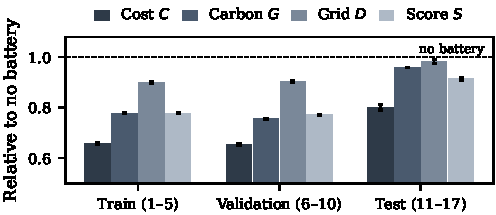
\includegraphics[width=\columnwidth]{fig_rltuned_kpis.pdf}
\caption{Cost, carbon, grid KPI and score of the RL-tuned MPC in each district, relative to no battery (dashed
line). Error bars show the standard deviation over three seeds.}
\label{fig:kpis}
\end{figure}

\subsection{Learned Behaviour}
To see what the controller has learned, we first look at the average day in the training district
(Fig.~\ref{fig:daily}). With no batteries, the district exports up to 5\,kW of PV at midday for nothing and imports about
6\,kW in the evening. Our controller stores it. The mean state of charge rises from under 10\% at dawn
to about 87\% at 14:00, and the batteries then discharge through the peak tariff from 16:00 to 21:00 and into the
night. As a result, the net load stays between about 0 and 4.5\,kW across the day, a much flatter profile for the grid.

\begin{figure}[!t]
\centering
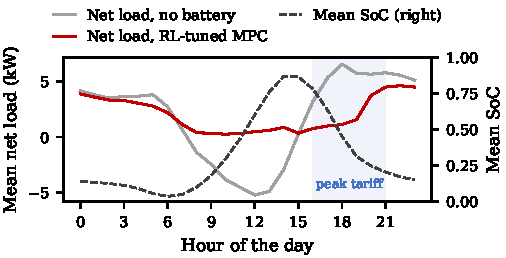
\includegraphics[width=\columnwidth]{fig_rltuned_daily.pdf}
\caption{Average daily profile over the year on the training buildings (seed 42): district net load with and without
batteries, and the mean state of charge.}
\label{fig:daily}
\end{figure}

A single July week (Fig.~\ref{fig:week}) shows the same daily pattern with one exception. On one day the controller
tops up from the grid in the last cheap hour before the peak tariff, and this creates a short import spike. Such spikes
cost little in $C$ and $G$. They do, however, raise the ramping and the monthly peak. This is the main reason why $D$
is our weakest KPI.

\begin{figure}[!t]
\centering
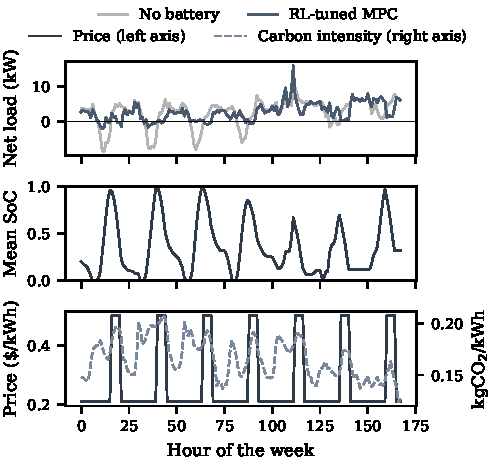
\includegraphics[width=\columnwidth]{fig_rltuned_week.pdf}
\caption{One July week on the training buildings (seed 42): district net load with and without batteries, mean state of
charge, and the price and carbon intensity.}
\label{fig:week}
\end{figure}

The learning curves in Fig.~\ref{fig:learning} are easy to read, because with the reward of (\ref{eq:reward}) the mean
reward per step is the weighted gain over idle batteries. Because we start the tuner from the weights of a good
fixed MPC, even the first, partly random year of training earns 0.84 per step, which is already far above zero. Over the next five simulated years the reward
rises by about 4\%. It then stays flat. One seed, 2026, levels off at a lower training reward, yet its public score
of 0.777 lies within one standard deviation of the others. We conclude that, once the solver handles the schedule, the
remaining differences in the weights matter little.

\begin{figure}[!t]
\centering
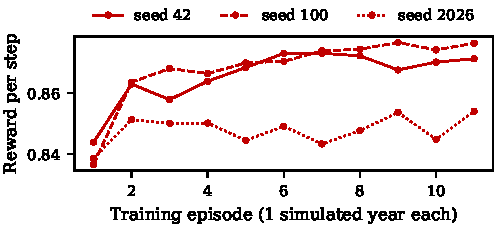
\includegraphics[width=\columnwidth]{fig_rltuned_learning.pdf}
\caption{Mean training reward per step of the RL weight tuner, three seeds. The reward is the weighted gain over no
battery, so zero means as good as idle batteries.}
\label{fig:learning}
\end{figure}

\subsection{Ablations}
In Table~\ref{tab:ablation} we change one component at a time. By far the largest loss came when we removed the
linear program. In that variant an RL agent with the same reward sets the battery rates directly. Even with history features and
twice the training, it reaches only $S = 0.862$ on buildings 1--5 and a public score of 0.854. The agent must then
learn from the reward the daily structure that the forecasts and the linear program would otherwise provide, and it
ramps more than idle batteries do ($D = 1.06$).

Replacing the RL tuner with the best fixed weights we found costs less, but the loss is consistent. With fixed
weights we obtain 0.781 on the public and 0.846 on the private board, against 0.774 and 0.844 with the tuner. Its
Phase~I score also rises from 0.717 to 0.742, and most of this difference comes from cost, which the tuner lowers
from 0.703 to 0.657 on the training homes at the price of slightly more ramping. In effect, the tuner learns when the
forecasts justify a more aggressive arbitrage.

The benefit of the tuner relies on reasonable forecasts. We replaced the LightGBM load and PV forecasts with seasonal
ones, using a 24-hour horizon. The controller still did well in the training district, with a Phase~I score of 0.728.
On new homes, however, it lost most of its advantage (public 0.807, private 0.864), since the agent had learned
weights that suit only the homes it was trained on. Tuning the LightGBM settings raises the PV accuracy from about 90\%
to 96\% and, at a 24-hour horizon, lowers the public score from 0.782 to 0.774. The horizon length and the RL
algorithm matter much less. Horizons of 24, 30 and 36 hours give public scores within 0.002 of each other. SAC in
place of TQC gives $0.775 \pm 0.001$.

\begin{table}[!t]
\centering
\caption{Ablations of the RL-tuned MPC, one change at a time (lower is better). Phase~I and $S$ on the training
homes, $S$ on the unseen validation and test buildings, and the Phase~III scores. Three seeds where marked $^\ast$,
otherwise seed 42.}
\label{tab:ablation}
\setlength{\tabcolsep}{2.5pt}
\resizebox{\columnwidth}{!}{%
\begin{tabular}{@{}lcccccc@{}}
\toprule
Variant & Phase I & $S_\mathrm{train}$ & $S_\mathrm{val}$ & $S_\mathrm{test}$ & Public & Private \\
\midrule
\textbf{Proposed (TQC, tuned LightGBM, 30 h)}$^\ast$ & 0.717 & 0.778 & \textbf{0.771} & 0.914 & \textbf{0.774} & \textbf{0.844} \\
\midrule
Fixed weights instead of RL tuning    & 0.742 & 0.784 & 0.779 & 0.910 & 0.781 & 0.846 \\
No solver: RL sets batteries$^\ast$ & 0.763 & 0.862 & 0.849 & --    & 0.854 & --    \\
Seasonal load and PV forecasts, 24 h  & 0.728 & 0.809 & 0.806 & 0.921 & 0.807 & 0.864 \\
Untuned LightGBM, 24 h$^\ast$          & 0.722 & 0.787 & 0.779 & \textbf{0.908} & 0.782 & 0.845 \\
Horizon 24 h                          & 0.723 & \textbf{0.777} & 0.772 & 0.913 & \textbf{0.774} & \textbf{0.844} \\
Horizon 36 h                          & 0.717 & 0.779 & 0.772 & 0.915 & 0.775 & 0.845 \\
SAC instead of TQC (36 h)$^\ast$       & \textbf{0.715} & 0.778 & 0.772 & 0.915 & 0.775 & 0.845 \\
\bottomrule
\end{tabular}}
\end{table}

\subsection{Comparison with the Challenge Leaderboards}
On the public leaderboard of the final phase, our controller would rank 8th of 42 (Fig.~\ref{fig:leader},
Table~\ref{tab:leader}). The leaderboard \cite{citylearn2022challenge} lists every entry's $C$, $G$ and $D$ as blends of
the training and validation districts. We use the same 0.4/0.6 blend for our row. Our score of 0.774 lies between
the 7th entry at 0.767 and the 8th at 0.789. The winner reached 0.728.

The ranking differs a good deal between the KPIs (Table~\ref{tab:kpirank}). Our carbon score of 0.764 is the lowest of
all 42 entries, 5\% below the best one (0.803). This holds for each of the three seeds. Our cost of 0.655 ranks 4th. Almost all of the gap to the top lies
in the grid KPI, where our $D$ of 0.902 ranks 14th and the winner reaches 0.738. Our reward weights carbon twice as much
as cost and gives up some grid smoothness for lower emissions. The carbon rank thus reflects this choice as much as the
quality of the controller.

\begin{figure*}[!t]
\centering
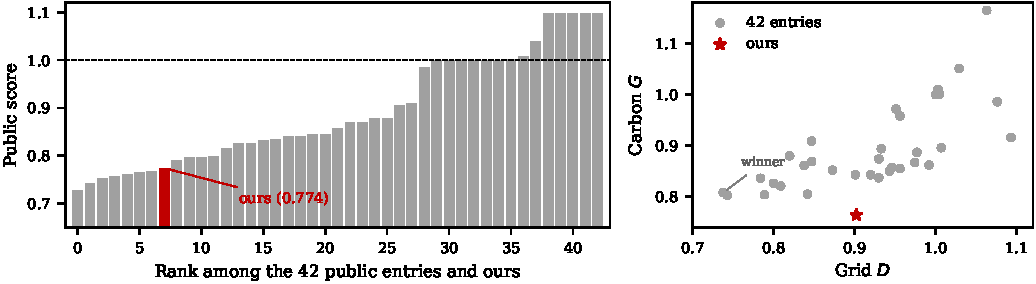
\includegraphics[width=\textwidth]{fig_leaderboard.pdf}
\caption{The proposed controller (dark bar and star) among the 42 entries of the Phase~III public leaderboard. Left: public scores in
rank order (dashed line: no battery). Right: carbon against grid KPI. No entry reaches lower emissions, but most
of the top entries have a smoother grid profile.}
\label{fig:leader}
\end{figure*}

The private leaderboard, which added the seven test buildings and decided the winners, was visible only to the
organisers, and its per-team values were never published. The challenge overview gives only the participants' medians
\cite{nweye2023challenge}, which are $C = 0.792$, $G = 0.940$, $D = 0.996$ and a score of 0.907. With the same private
weights of 0.2, 0.3 and 0.5, our controller reaches $C = 0.728$, $G = 0.861$, $D = 0.942$ and a score of 0.844. It
beats the median on every KPI. We cannot check whether its carbon is also the lowest on the private leaderboard.

The Phase~I leaderboard scored $(C+G)/2$ on the training buildings, and its best entries reached 0.631, 0.635 and
0.651. Our 0.717 would rank 5th. During that phase, however, the teams had the full year of these homes and could
optimise on the actual data, as the runner-up did with dynamic programming \cite{nweye2023challenge}. For
this reason we regard the final phase, on homes no team had seen, as the fairer comparison.

\begin{table}[!t]
\centering
\caption{Phase~III public leaderboard (top 8 of the 42 entries) with the proposed controller (mean of three seeds).}
\label{tab:leader}
\resizebox{\columnwidth}{!}{%
\begin{tabular}{@{}clcccc@{}}
\toprule
Rank & Team & Score & $C$ & $G$ & $D$ \\
\midrule
1 & Together           & \textbf{0.728} & \textbf{0.639} & 0.808 & \textbf{0.738} \\
2 & ambitiousengineers & 0.742 & 0.681 & 0.803 & 0.743 \\
3 & CUFE               & 0.753 & 0.665 & 0.804 & 0.789 \\
4 & EVERGi\_team       & 0.756 & 0.643 & 0.826 & 0.800 \\
5 & Orca               & 0.760 & 0.659 & 0.836 & 0.784 \\
6 & Greener            & 0.764 & 0.663 & 0.821 & 0.809 \\
7 & DivMARL            & 0.767 & 0.653 & 0.805 & 0.842 \\
-- & \textit{Ours: RL-tuned MPC} & \textit{0.774} & \textit{0.655} & \textbf{\textit{0.764}} & \textit{0.902} \\
8 & SCRG\_UA           & 0.789 & 0.666 & 0.880 & 0.820 \\
\bottomrule
\end{tabular}}
\end{table}

\begin{table}[!t]
\centering
\caption{Rank of the RL-tuned MPC on each KPI among the 42 entries of the Phase~III public leaderboard.}
\label{tab:kpirank}
\resizebox{\columnwidth}{!}{%
\begin{tabular}{@{}lccl@{}}
\toprule
Indicator & Best of 42 entries & Ours & Our rank \\
\midrule
Carbon $G$ & 0.803 (ambitiousengineers) & \textbf{0.764} & \textbf{1st} \\
Cost $C$   & 0.639 (Together) & 0.655 & 4th \\
Grid $D$   & 0.738 (Together) & 0.902 & 14th \\
Overall    & 0.728 (Together) & 0.774 & between 7th and 8th \\
\bottomrule
\end{tabular}}
\end{table}

\subsection{Where the Remaining Gap Lies}\label{sec:fcvalue}
Among the quantities we forecast, the load is by far the most difficult to predict (Table~\ref{tab:fc}). We measure accuracy as one
minus the mean absolute error over the mean load. With LightGBM, a single home's hourly load is 50--59\% predictable,
only a little better than with the seasonal rule. The district total is far easier, at 71--78\%, because the random
swings of the homes partly cancel, and this total is also what the grid KPIs and the clipped cost see. For PV, by contrast,
we reach about 96\% accuracy.

\begin{table}[!t]
\centering
\caption{Load forecast accuracy over the next 24 hours ($1 -$ MAE / mean, \%), per building and for the district total.}
\label{tab:fc}
\resizebox{\columnwidth}{!}{%
\begin{tabular}{@{}lcccc@{}}
\toprule
 & \multicolumn{2}{c}{Per building} & \multicolumn{2}{c}{District total} \\
\cmidrule(lr){2-3}\cmidrule(l){4-5}
District & Seasonal & LightGBM & Seasonal & LightGBM \\
\midrule
Train (1--5)       & 54.5 & \textbf{58.3} & 74.7 & \textbf{75.0} \\
Validation (6--10) & 45.1 & \textbf{50.1} & 69.3 & \textbf{70.6} \\
Test (11--17)      & 57.6 & \textbf{58.7} & \textbf{78.4} & 77.5 \\
\bottomrule
\end{tabular}}
\end{table}

To find which errors cost score, we gave the fixed-weight version of the controller the true future for one part of its
forecasts at a time (Fig.~\ref{fig:fcvalue}). Since this test uses the future, it only bounds what better forecasts
could give. For reference, with its own forecasts the controller scores $S = 0.784$ in the training and 0.779 in the validation
district. Perfect PV forecasts change almost nothing (0.782 and 0.776), whereas perfect load forecasts lower $S$
to 0.648 in both districts, which is well below the level that the winner of the challenge reached.

Nearly all of this value lies in the district total over the next few hours, since rescaling the building forecasts
to the true district total already lowers $S$ to 0.649 and 0.648. Giving the true load for only the next six hours yields 0.659 and
0.651. The remaining gap is therefore due mainly to the hourly forecast of the district's total load. It is not due to
the solver or the tuner.

\begin{figure}[!t]
\centering
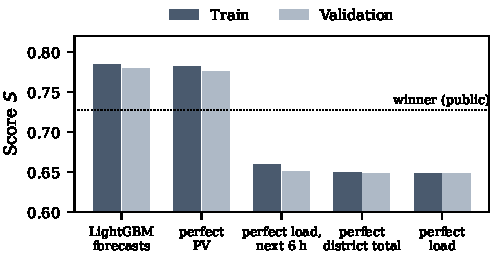
\includegraphics[width=\columnwidth]{fig_forecast_value.pdf}
\caption{Score of the fixed-weight controller when one part of its forecasts is replaced by the true future (an upper
bound). The dotted line marks the winner's public score.}
\label{fig:fcvalue}
\end{figure}

\section{Discussion}\label{sec:discussion}
In our design, RL is more useful as a tuner of the optimiser than as the controller itself. The agent does not have to
discover the daily patterns of price, PV and demand, or the physics of the batteries, because the forecasts and the
linear program supply both. Its three actions only shift a schedule that is already sensible, so a credit-assignment problem over thousands of
hourly battery decisions becomes a much easier one. This explains why removing the solver
costs far more (public 0.854) than removing the tuner (0.781). The tuning pays off only with good forecasts. With seasonal ones, the agent fitted its weights to the training homes
and lost most of its advantage on new ones.

We trail the winner mainly in the grid KPI, where we reach $D = 0.902$ on the public blend and the winner 0.738.
Short import spikes, such as a top-up in the last cheap hour before the peak tariff (Fig.~\ref{fig:week}), are cheap
in cost and carbon. In ramping and load factor, they are costly. We see two remedies: a load-factor term in the linear
program, and better forecasts of the district total, which Section~\ref{sec:fcvalue} identifies as the quantity that
matters most. We leave both for future work. Because the inputs of the tuner are district-level, the controller also runs on new districts of a
different size without retraining. It could therefore serve as a starting point that is fine-tuned on site.

Our study has several limitations. It covers one climate and one year of data, with five training buildings, and the
environment does not forecast carbon intensity or load. We compute the scores with the official formulas on CityLearn
2.1.2 rather than with the challenge's evaluator. The weather ``forecasts'' of the data equal the actual weather,
although every entry received the same data. Three seeds give reliable means for the proposed controller, with standard
deviations of at most 0.006, but most ablations use one seed. Hourly household load also remains hard to forecast, and
better inputs, such as occupancy, appliance schedules or sub-hourly data, are more likely to help than larger models.
Beyond these results, the work serves several of the United Nations Sustainable Development Goals (SDGs), which
Table~\ref{tab:sdg} lists in order of relevance.

\begin{table}[!t]
\centering
\caption{United Nations Sustainable Development Goals addressed by this work.}
\label{tab:sdg}
\footnotesize
\renewcommand{\arraystretch}{1.25}
\begin{tabular}{@{}>{\raggedright\arraybackslash}p{2.6cm}>{\raggedright\arraybackslash}p{5.6cm}@{}}
\toprule
SDG & Justification \\
\midrule
SDG 13 (Climate Action) &
A carbon weight retuned every hour cuts CO$_2$ emissions by 22\% and gives the lowest carbon score of all leaderboard
entries. \\
SDG 7 (Affordable and Clean Energy) &
Cuts electricity bills by about a third and stores rooftop PV surplus that would otherwise be exported for nothing. \\
SDG 11 (Sustainable Cities and Communities) &
Coordinates the batteries of a whole district and smooths the load that the local grid supplies. \\
SDG 9 (Industry, Innovation and Infrastructure) &
Shows an AI control design for smart energy infrastructure. \\
SDG 12 (Responsible Consumption and Production) &
Shifts consumption toward cheaper, lower-carbon hours. \\
\bottomrule
\end{tabular}
\end{table}

\section{Conclusion}\label{sec:conclusion}
We proposed an RL-tuned model predictive controller for community battery storage. In our design, LightGBM forecasts
drive a receding-horizon linear program, and a TQC agent retunes its ramping, carbon and storage weights every hour from
district-level features. The agent learns from a reward that adds up to the KPIs. On the CityLearn 2022 benchmark the
controller cut the electricity cost by 34.3\% and the emissions by 22.2\% in the training district. Over three seeds it
reached a public score of $0.774 \pm 0.003$ and a private score of $0.844 \pm 0.004$, between 7th and 8th place on the
public leaderboard. Its carbon score of 0.764 is the lowest of all 42 entries. Every private KPI also beats the participants'
median.

Our ablations show that the solver contributes most and that the RL tuning adds a steady gain once the forecasts are
good. Neither the horizon nor the choice of RL algorithm changed the public score by more than 0.002. What remains
between us and the winner lies in the grid KPI and, above all, in the forecast of the district's total load over the
next few hours. With perfect load forecasts, the same solver would score about 0.65. For practical systems, we would
therefore align the reward with the evaluation, use RL to adapt an optimiser rather than to replace it, and invest in
better forecasts.

\bibliographystyle{IEEEtran}
\bibliography{references}

\end{document}
